%!TEX root = Slic3r-Manual.tex

\section{Impression S\'equentielle} % (fold)
\label{sec:sequential_printing}
\index{Sequential Printing}
\index{Impression S\'equentielle}

Lors de l'impression de plusieurs objets \`a la fois, il peut \^etre utile d'imprimer chacun s\'epar\'ement, ce qui r\'eduira le suintement et les ficelles se formant entre les impressions. Cela permettra aussi de r\'eduire le risque qu''un probl\`eme ne ruine toute l'impression - si une partie se d\'etache ou \'echoue d'une certaine mani\`ere, il ne sera pas tra\^in\'e dans d'autres parties de l'impression \`a chaque couche.

\begin{figure}[H]
\centering
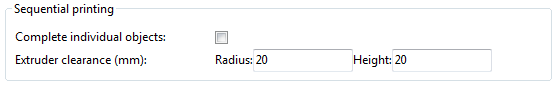
\includegraphics[keepaspectratio=true,width=1\textwidth]{simple_mode/sequential_printing_options.png}
\caption{Options d'impression s\'equentielle.}
\label{fig:sequential_printing_options}
\end{figure}

\index{Print Settings!Output options!Sequential printing!Extruder clearance}
\index{Param\`etres d'Impression!Options de sortie!Impression s\'equentielle!D\'egagement de l'extrudeuse}
Un soin doit \^etre pris afin que la buse et extrudeuse n'interf\`ere pas avec les parties d\'ej\`a imprim\'ees.  Slic3r devrait avertir s'il d\'etecte que la buse ou l'extrudeuse peuvent entrer en collision avec une pi\`ece, mais v\'erifiez que la disposition des pi\`eces ne puisse pas causer de probl\`eme.  Le param\`etre \texttt{Extruder clearance} (D\'egagement de l'extrudeuse) aide Slic3r \`a d\'etecter les risques de collision:
\begin{itemize}
	\item \texttt{Radius} (Rayon) - Le d\'egagement qui devrait \^etre accord\'ee autour de l'extrudeuse. Prenez soin si l'extrudeuse n'est pas mont\'e au centre - prendre la plus grande valeur par s\'ecurit\'e.
	\item \texttt{Height} (Hauteur) - La distance verticale entre la buse et les tiges de l'axe X, ou partie la plus basse qui peut interf\'erer avec une impression finale.
\end{itemize}

\begin{figure}[H]
\centering
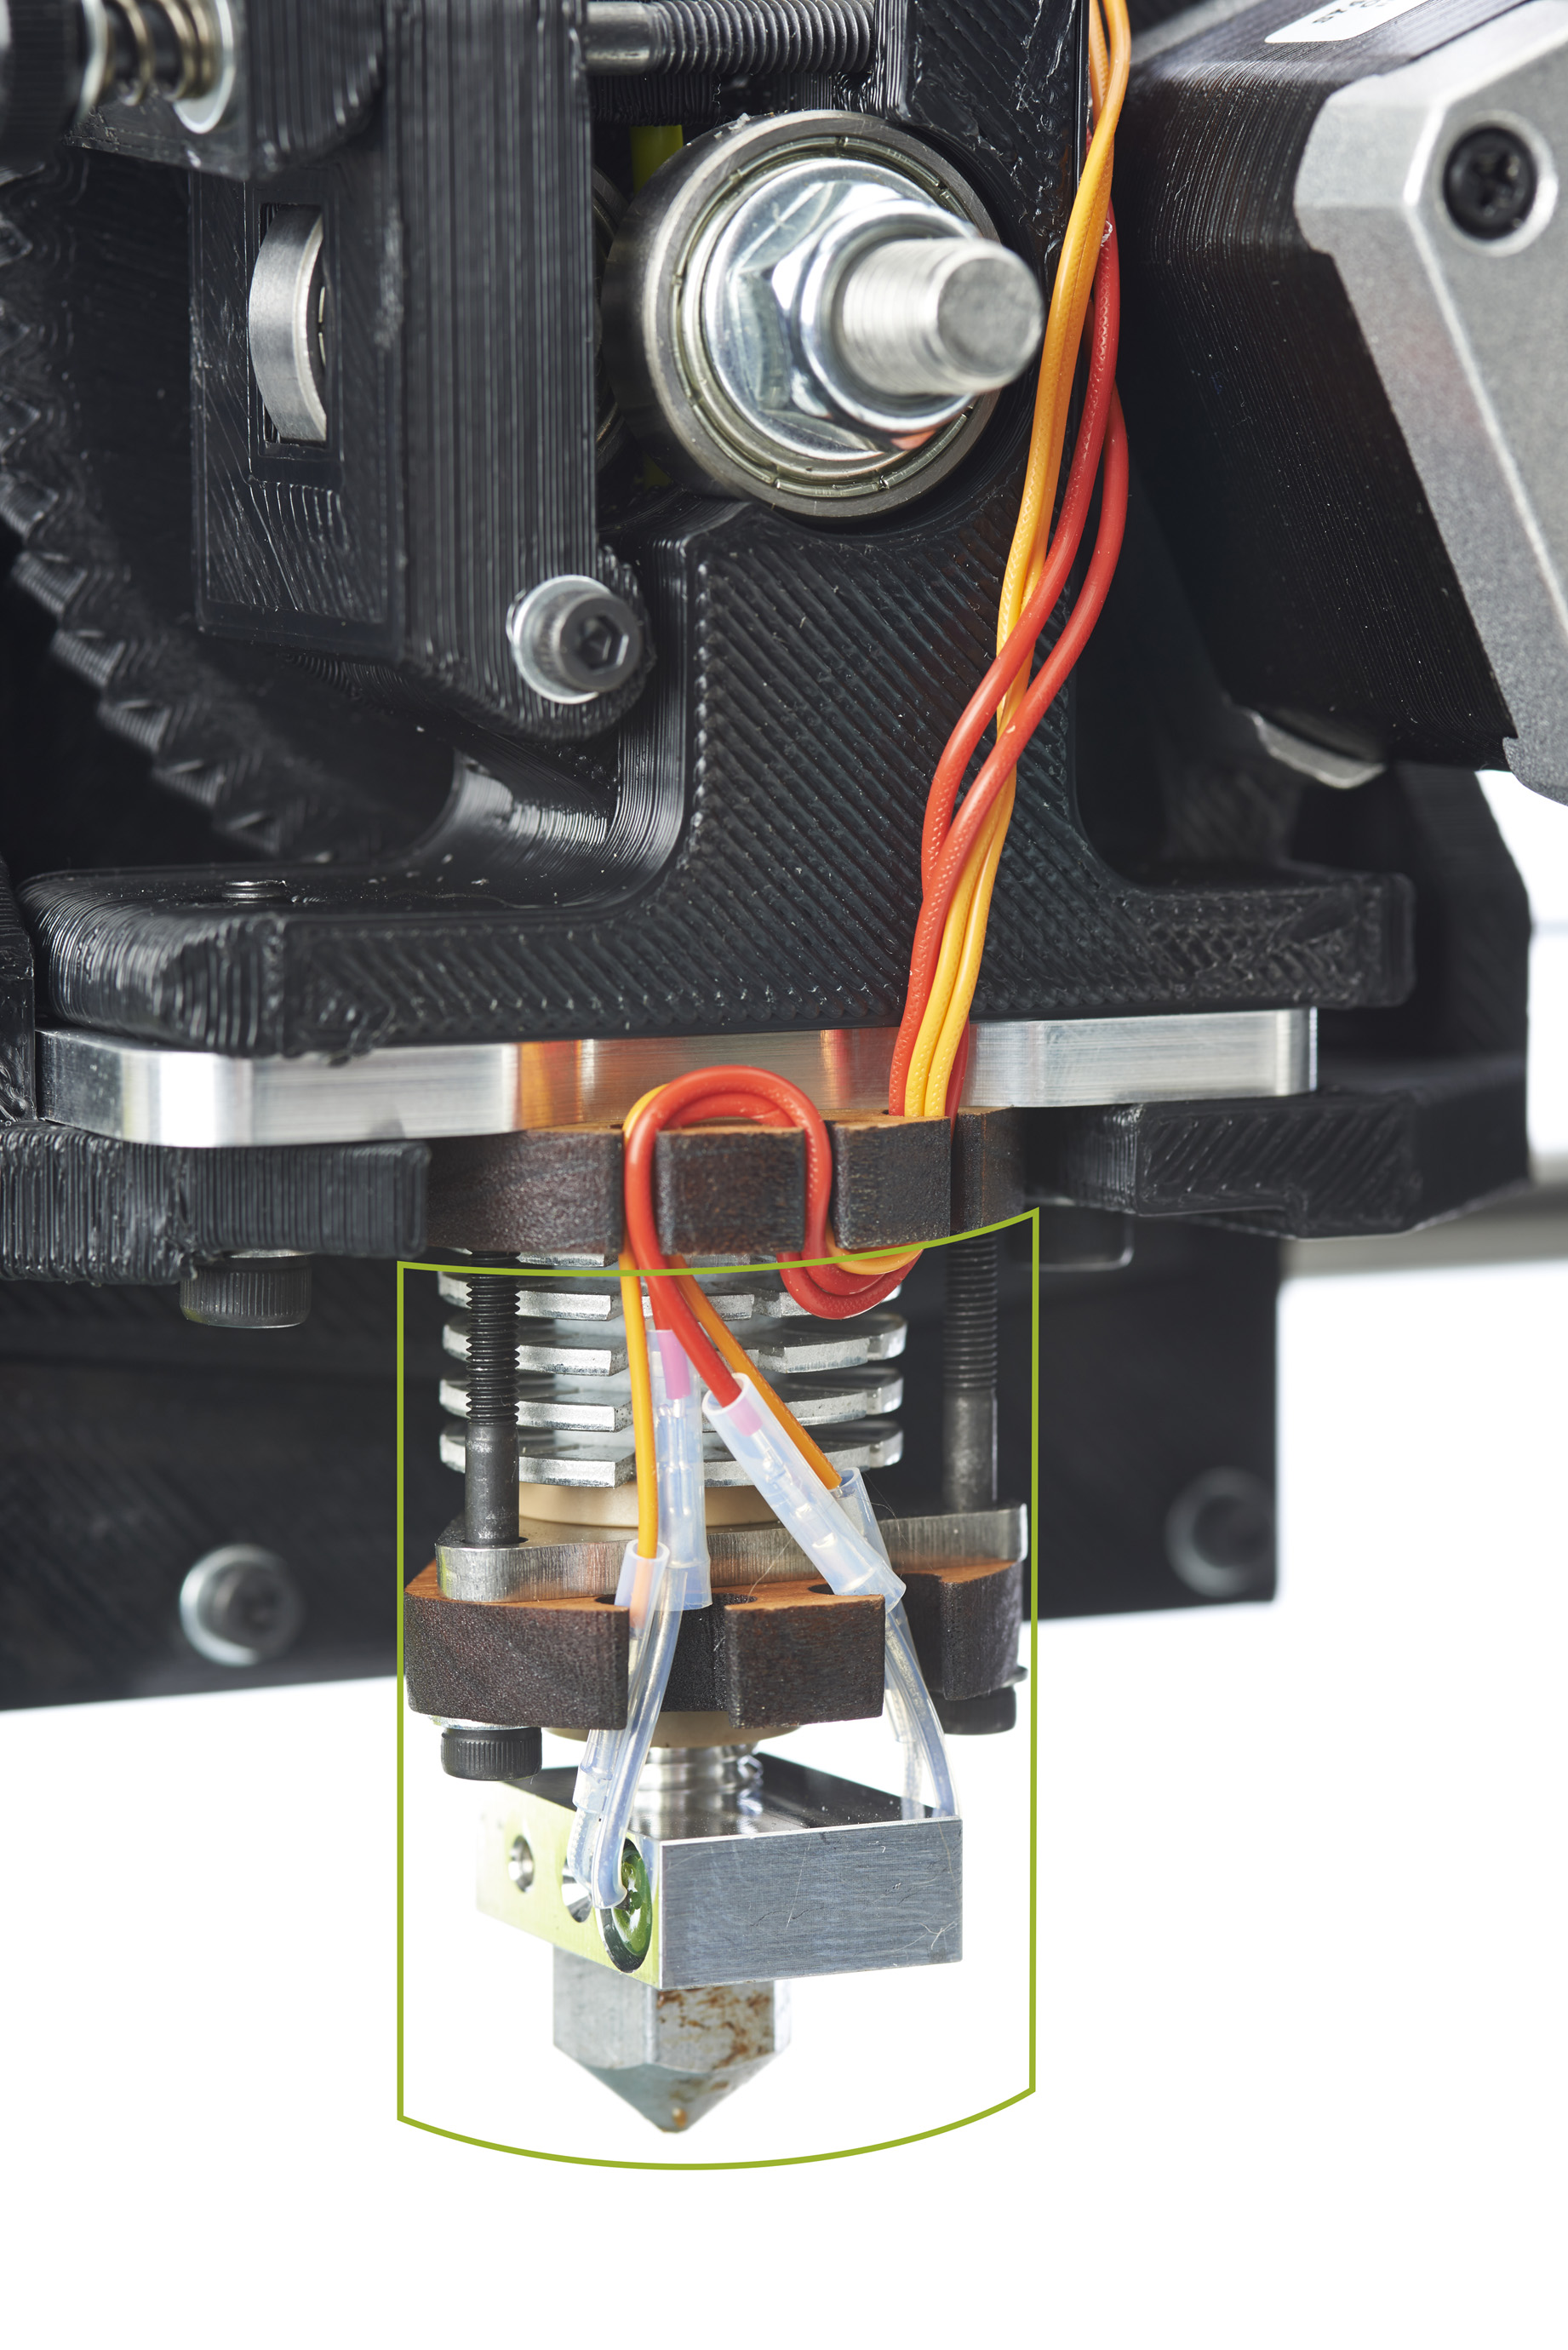
\includegraphics[keepaspectratio=true,width=0.5\textwidth]{simple_mode/extruder_clearance.jpg}
\caption{Le cylindre de d\'egagement autour de l'extrudeuse.}
\label{fig:a_diagram_depicting_extruder_clearance}
\end{figure}

